\section{Theorie}
\label{sec:Theorie}

\subsection{Der Rutherford'sche Streuversuch mit Americium-Quelle}
Beim Rutherford'schen Streuversuch werden $\alpha$-Teilchen auf eine dünne Goldfolie geschossen und die Anzahl der gestreuten Teilchen in Abhängigkeit vom Streuwinkel $\theta$ gemessen.\\
Die $\alpha$-Teilchen werden aus dem Zerfall eines radioaktiven Isotops, hier $^{241}.{Am}$, gewonnen:
\[
^{241}_{95}.{Am}\rightarrow ^{237}_{93}.{Np} + ^{4}_{2}.{\alpha}\text{.}
\]
Die möglichen Übergänge dieser Reaktion mit verschieden angeregten $^{237}_{93}.{Np}$-Endprodukten sind in Abbildung \ref{fig:uebergang} zu sehen. Der dominante Prozess ist der hier mit $\alpha_.3$ bezeichnet. Der Anteil an $\alpha$-Strahlung durch weiteren Zerfall des Neptuniums kann auf Grund seiner wesentlich höheren Halbwertszeit vernachlässigt werden.\\
\begin{figure}
\centering
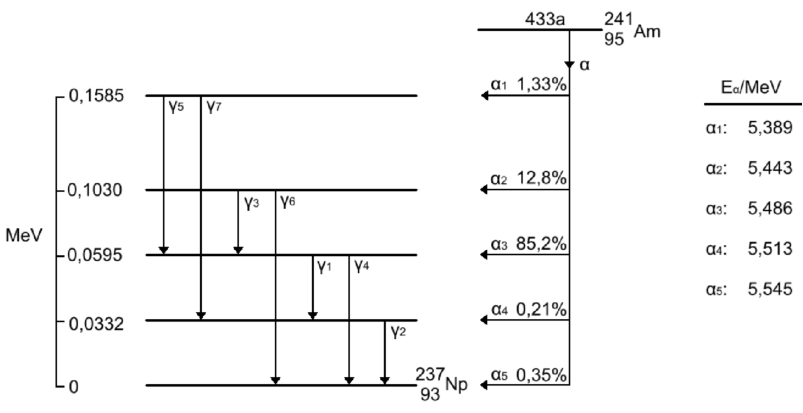
\includegraphics[width=\linewidth-60pt,keepaspectratio]{content/images/uebergang.pdf}
\caption{Übergangsschema des Isotops $^{241}_{95}.{Am}$ \cite{Schema16}.}
\label{fig:uebergang}
\end{figure}

\subsection{Wechselwirkung geladener Teilchen mit Materie}
\noindent Wechselwirkt ein geladenes Teilchen mit einer Masse $m\gg m_.e$, wobei $m_.e$ die Elektronenmasse ist, in Materie, so gibt es zwei Möglichkeiten der Wechselwirkung.
Entweder das Teilchen wechselwirkt mit den Hüllenelektron, auf Grund des großen Massenunterschieds wird dabei zwar Energie abgegeben, jedoch ändert sich seine Flugrichtung nicht. Die andere Möglichkeit ist eine Wechselwirkung mit dem Coulombpotential des Kerns. Da ein $\alpha$-Teilchen zweifach positiv geladen ist, wird es stark aus seiner Bahn ausgelenkt und gibt nur einen kleinen Teil seiner Energie in Form von Bremsstrahlung an das Medium ab.
Auf Grund der Ausdehnung der Materie kommt es zu sehr vielen Wechselwirkungen, wobei der Energieverlust pro Wegstrecke eines einfallenden $\alpha$-Teilchens gegeben ist durch die Bethe-Bloch-Formel für niedrige Energien
\begin{equation}
\frac{\mathrm{d}E}{\mathrm{d}x}=\frac{4\pi e^4z^2n Z}{m_.ev^2(4\pi\epsilon_.0)^2}\log{\left(\frac{2m_.ev^2}{I}\right)}\text{.}\label{eq:BBF}
\end{equation} 
Dabei ist $e$ die Elementarladung, $z=2$ die Ladungszahl des $\alpha$-Teilchens, $Z$ die Kernladungszahl der Atome des Mediums, $n$ die Anzahl der Atome pro $\si{\centi\meter^3}$, $v$ die Geschwindigkeit des $\alpha$-Teilchens und $I=(\SI{10}{\electronvolt})Z$ die mittlere Ionisationsenergie. Umformen nach $dx$ ergibt für die Schichtdicke
\begin{equation}
dx=dE\frac{4\pi m_.e v^2\epsilon^2_.0}{e^4z^2nZ}\log^{-1}\left(\frac{2m_.e v^2}{I}\right)\text{.}\label{eq:dx}
\end{equation}
Für das Bremsvermögen in Luft genähert als Stickstoff kann das Geschwindigkeitsquadrat näherungsweise über $v^2=\frac{2E_.{\alpha}}{m_.{\alpha}}$ mit Energie und Masse des $\alpha$-Teilchens $E_.{\alpha}$ und $m_.{\alpha}$ beschrieben werden. Somit ergibt sich mit den Werten $n_.N = \SI{2,69e25}{\metre^{-3}}$, $Z_.N=7$, $I_.N=\SI{70}{\electronvolt}$, $m_.{\alpha}=\SI{6,64e-27}{\kilo\gram}$, $z_.{\alpha}=2$ und der Energie $E_.{\alpha}=\SI{5,486}{\mega\electronvolt}$ aus Abbildung \ref{fig:uebergang}:
\begin{equation*}
\left(\frac{dE}{dx}\right)_.{N}=\SI{0,40}{\mega\electronvolt}\text{.}
\end{equation*}

\subsection{Der Rutherford'sche Wirkungsquerschnitt}
Der Wirkungsquerschnitt $\sigma$ ist ein Maß für die Wahrscheinlichkeit der Wechselwirkung des $\alpha$-Teilchens im Medium.
Der differentielle Wirkungsquerschnitt pro Raumwinkelelement $\frac{\mathrm{d}\sigma}{\mathrm{d}\Omega}$ ist gegeben durch die Rutherford-Streuformel
\begin{equation}
\frac{\mathrm{d}\sigma}{\mathrm{d}\Omega}(\theta)=\frac{1}{(4\pi\epsilon)^2}\left(\frac{z Z e^2}{4 E_.{\alpha}}\right)^2\frac{1}{\sin^4{\left(\frac{\theta}{2}\right)}},\label{eq:RSF}
\end{equation}
wobei $E_.{\alpha}$ die mittlere Energie des $\alpha$-Teilchens ist. Auch diese Formel gilt nur für niedrige Energie, da sonst die Form der Kerne über Formfaktoren berücksichtigt werden müssen.
Der Gesamtwirkungsquerschnitt ergibt sich durch Aufsummieren der differentiellen Wirkungsquerschnitte und infinitesimal ergibt sich damit
\[
\sigma = \int \frac{\mathrm{d}\sigma}{\mathrm{d}\Omega}\mathrm{d}\Omega\text{.}
\]
Auf Grund der geringen Reichweite von $\alpha$-Strahlung in Luft, wird eine Vakuumkammer um den Versuch herum benötigt.






%±♦◘♥
